\documentclass[conference]{IEEEtran}

% ---------------------------------------------------------
% PACKAGES
% ---------------------------------------------------------
\usepackage{cite}
\usepackage{amsmath,amssymb,amsfonts}
\usepackage{algorithmic}
\usepackage{graphicx}
\usepackage{textcomp}
\usepackage{xcolor}
\usepackage{booktabs}
\usepackage{multirow}
\usepackage{url}
\usepackage{float}
\usepackage{array}
\usepackage{balance}
\usepackage{siunitx}
\usepackage{titlesec}
\usepackage{lscape}

% Reduce spacing around figures and section
\setlength{\abovecaptionskip}{6pt}
\setlength{\belowcaptionskip}{6pt}
\setlength{\textfloatsep}{12pt}
\setlength{\intextsep}{12pt}
\setlength{\parskip}{0pt}

% Tighten section spacing
\titlespacing{\section}{0pt}{12pt}{6pt}
\titlespacing{\subsection}{0pt}{10pt}{4pt}
\titlespacing{\subsubsection}{0pt}{8pt}{2pt}

% ---------------------------------------------------------
% DOCUMENT
% ---------------------------------------------------------
\begin{document}

\title{Multi-Modal Periodic Energy-Based Navigation System for Autonomous Drone Homing}

% ---------------------------------------------------------
% AUTHORS
% STUDENTS FIRST, GUIDES/FACULTY SECOND
% ---------------------------------------------------------
\author{
\IEEEauthorblockN{
Sreejith S., Jaijan S., P. L. Vijaya Vittal, P. L. V. Karthik
}
\IEEEauthorblockA{
Student Authors\\
Department of Information Science and Engineering\\
Department of Artificial Intelligence and Machine Learning\\
Department of Electronics and Communication Engineering\\
Cambridge Institute of Technology, Bengaluru, India
}
\and
\IEEEauthorblockN{
Dr. Preethi S., Dr. M. Varalatchoumy, Dr. Nagesh K. N.
}
\IEEEauthorblockA{
Faculty Guides\\
Department of Information Science and Engineering\\
Department of Artificial Intelligence and Machine Learning\\
Department of Electronics and Communication Engineering\\
Cambridge Institute of Technology, Bengaluru, India
}
}

\maketitle
% =========================================================
% ABSTRACT
% =========================================================

\begin{abstract}
Autonomous drone homing remains challenging when Global Navigation Satellite
System (GNSS) signals are unavailable, obstructed, jammed, or unreliable.
This paper presents a multi-modal periodic energy-based navigation system that
combines optical, thermal, and acoustic sensing in a staged GPS-independent
homing architecture. A designated base station periodically emits identifiable
signals in multiple physical modalities. During the long-range phase, optical
and thermal measurements provide coarse target direction; during the near-field
phase, a microphone array provides acoustic localization using Time Difference
of Arrival (TDOA), Angle of Arrival (AOA), and signal-strength information.
The architecture integrates signal acquisition, filtering, feature extraction,
sensor fusion, localization, navigation, flight control, telemetry, and safety
monitoring in a closed loop. A web-based ground-control layer supports live
telemetry, mission replay, event logging, and health monitoring. The prototype
and development workflow are evaluated using signal-processing, localization,
integration, telemetry, and replay-oriented metrics. The reported numerical
values are development/replay observations rather than final free-flight
measurements. The work provides a practical architecture for future
hardware-in-the-loop and controlled flight validation in GPS-denied environments.
\end{abstract}

\begin{IEEEkeywords}
Autonomous Drone, GPS-Free Navigation, Drone Homing, Sensor Fusion,
Optical Sensing, Thermal Sensing, Acoustic Localization, TDOA, AOA,
Periodic Beacon, UAV Navigation.
\end{IEEEkeywords}

% =========================================================
% I. INTRODUCTION
% =========================================================

\section{Introduction}

Unmanned Aerial Vehicles (UAVs) are increasingly used for inspection,
surveillance, logistics, environmental monitoring, disaster response, and
autonomous exploration. Reliable localization is fundamental to these
applications because the navigation stack must continuously estimate the
vehicle state and generate safe motion commands
\cite{mahony2012,floreano2015,faessler2018,mellinger2011}. Conventional outdoor
autonomous flight frequently relies on GNSS/GPS for global position and
return-to-home functions. However, satellite-based positioning can degrade or
become unavailable indoors, underground, beneath structures, in dense urban
canyons, or under intentional interference
\cite{jarraya2025,vanegas2016,skjetne2011}.

Vision-based navigation and visual-inertial odometry can provide rich geometric
information, but feature extraction and tracking may degrade under low light,
smoke, dust, blur, occlusion, repetitive texture, or other visual degradation
\cite{leutenegger2015,forster2017,campos2021,orbslam3}. LiDAR and camera fusion
can improve geometric robustness, but additional sensing hardware increases
payload, computation, calibration effort, and system complexity
\cite{quach2026}. RF and ultra-wideband (UWB) systems can provide absolute or
relative positioning when infrastructure is available, but their performance
can be affected by multipath, propagation conditions, anchor geometry, and
interference
\cite{zafari2019,schwarz2017,liu2014,wang2024}. Acoustic localization is
attractive for short-range directional estimation and can use microphone arrays
with TDOA/GCC-based processing, but ambient noise, reverberation, reflections,
and array geometry affect accuracy
\cite{brandstein2001,knapp1976,chen2006,do2010}.

Thermal sensing provides complementary information in conditions where visible
imagery is weak or illumination is poor, and UAV research has explored thermal
imagery for localization and perception in challenging environments
\cite{jensen2007,flir2018,thermal2026}. The broader GNSS-denied navigation
literature increasingly emphasizes sensor fusion because no single modality is
robust under all environmental conditions
\cite{jarraya2025,alqudsi2026}. Kalman filtering and probabilistic state
estimation are widely used to combine measurements with different uncertainty,
rates, and failure modes
\cite{welch1995,maybeck1979,barshalom2001,thrun2005}.

These observations motivate a staged multi-modal strategy rather than a single
estimator operating identically throughout the mission. The proposed system
uses a designated periodic beacon as an explicit homing reference. Optical and
thermal measurements are used for long-range target acquisition, while acoustic
TDOA/AOA information is activated for near-field refinement. The design
therefore assigns each modality to the region where it is most useful, while a
fusion layer controls the contribution of each measurement according to
confidence and signal quality. The architecture also couples localization to
navigation state, flight control, telemetry, and safety rather than treating
localization as an isolated module
\cite{gustafsson2012,mahony2012,lee2010}.

% ---------------------------------------------------------
% RESEARCH GAP
% ---------------------------------------------------------

\subsection{Research Gap}

Existing GPS-denied UAV solutions commonly optimize a dominant modality such as
vision, inertial sensing, LiDAR, UWB, or acoustics. Such systems can perform
well under their intended conditions, but their failure modes differ. Vision
can be weakened by illumination and scene degradation; RF/UWB systems require
appropriate infrastructure and are sensitive to propagation conditions;
acoustic systems are most useful at shorter ranges and can be affected by
reverberation; and inertial estimation accumulates drift without external
correction
\cite{vanegas2016,leutenegger2015,orbslam3,zafari2019,brandstein2001,faessler2018}.

The research gap addressed by this work is therefore the lack of a compact,
staged homing architecture that deliberately combines periodic optical,
thermal, and acoustic energy cues, switches modalities according to the
estimated homing phase, and connects the resulting localization to a complete
navigation, control, telemetry, and safety loop. The contribution is not the
invention of any individual sensing technique; rather, it is the system-level
integration and staged use of complementary physical modalities for a
designated GPS-independent homing task.

% =========================================================
% II. RELATED WORK
% =========================================================

\section{Related Work}

GPS-based UAV navigation provides reliable global positioning and is widely
used for autonomous flight and return-to-home functions. However, its
dependence on satellite visibility limits operation in indoor, obstructed,
underground, and intentionally denied environments
\cite{vanegas2016,px4guide,px4return}. Vision-based navigation and
visual-inertial systems provide rich environmental information and can support
localization without GNSS, but their performance depends on illumination,
texture, feature availability, computational resources, and scene conditions
\cite{leutenegger2015,forster2017,orbslam3,faessler2018}.

RF and UWB approaches provide useful relative or absolute localization when
suitable infrastructure is available. Their accuracy can nevertheless depend
on anchor geometry, multipath, propagation conditions, and interference
\cite{zafari2019,liu2014,wang2024}. Acoustic localization provides another
alternative, particularly for directional and short-range localization.
Microphone arrays combined with TDOA, GCC, and AOA processing can estimate
source direction, although noise, reverberation, reflections, and microphone
geometry influence accuracy
\cite{brandstein2001,knapp1976,chen2006,do2010}.

Multi-sensor fusion provides a means of combining complementary measurements
and reducing dependence on a single sensing modality
\cite{welch1995,barshalom2001,gustafsson2012}. The proposed work extends this
principle to a designated periodic homing reference by assigning optical and
thermal sensing to long-range target acquisition and acoustic localization to
near-field refinement. This staged organization connects sensing, localization,
navigation, control, telemetry, and safety within one GPS-independent homing
workflow.

% =========================================================
% III. PROBLEM STATEMENT AND OBJECTIVES
% =========================================================

\section{Problem Statement and Objectives}

\subsection{Problem Statement}

The problem considered in this work is the autonomous return of a UAV toward a
designated base station when GNSS/GPS cannot be assumed to be continuously
available. The drone must detect the base-station beacon, estimate its relative
direction and/or position, select an appropriate navigation mode, generate
flight-control commands, and continue the measurement--decision--motion loop
until target alignment is achieved. The system must also tolerate changes in
signal quality and provide a safe response to localization uncertainty,
communication loss, or sensor failure.

The design is intentionally reference-based: the base station provides a known
periodic source rather than requiring a pre-built global map. This makes the
problem suitable for indoor recovery, structured GPS-denied areas, controlled
search-and-rescue scenarios, and other deployments where a homing reference can
be installed
\cite{vanegas2016,achtelik2009,jarraya2025}.

\subsection{Objectives}

The primary objective is to develop a GPS-independent UAV homing architecture
that combines optical, thermal, and acoustic sensing with a periodic beacon.
The system is designed to use optical and thermal measurements for long-range
target acquisition, followed by microphone-array TDOA/AOA processing for
near-field directional refinement. A confidence-aware fusion mechanism is
intended to combine heterogeneous observations according to signal quality and
uncertainty. The navigation layer connects localization estimates to navigation
states and PID-based flight-control commands, while the telemetry and
ground-control layer provides mission monitoring, replay, event logging, and
safety supervision. The complete workflow is evaluated using signal,
localization, integration, telemetry, and homing-performance metrics while
clearly distinguishing development and replay observations from future
physical-flight measurements.

% =========================================================
% IV. PROPOSED METHODOLOGY
% =========================================================

\section{Proposed Methodology}

The proposed methodology is organized as a closed-loop pipeline:

{\small
\begin{center}
\textbf{Base Station}
$\rightarrow$
\textbf{Sensors}
$\rightarrow$
\textbf{Signal Processing}
$\rightarrow$
\textbf{Sensor Fusion}
$\rightarrow$
\textbf{Localization}
$\rightarrow$
\textbf{Navigation}
$\rightarrow$
\textbf{Flight Control}
$\rightarrow$
\textbf{Actuation}.
\end{center}
}

% ---------------------------------------------------------
% SYSTEM ARCHITECTURE
% ---------------------------------------------------------

\subsection{System Architecture and Overall Flow}

The proposed system follows a layered architecture consisting of a base-station
layer, onboard sensor layer, signal-processing layer, localization and fusion
layer, navigation and decision layer, flight-control layer, telemetry layer,
and safety layer. This separation permits individual modules to be tested
independently before complete system integration. The architecture follows
established UAV and robotics system-modeling principles
\cite{corke2017,siciliano2016,spong2006} while adapting the localization source
to a dedicated multi-modal homing beacon
\cite{mahony2012,lee2010,corke2017,px4guide}.

The overall operation begins at the base station, which periodically generates
identifiable energy cues. The drone sensor layer acquires these signals and
passes them to the signal-processing stage. Filtering, frequency analysis,
feature extraction, and noise suppression are then performed independently for
each sensing modality. The resulting features are passed to the fusion layer,
where confidence and signal-quality information determine the contribution of
each modality.

The localization layer converts the fused measurements into target direction
or relative position. The navigation layer interprets this estimate according
to the current homing state and generates the required movement direction. The
flight-control layer converts these navigation commands into attitude and
throttle corrections, which are finally executed through the flight controller,
ESCs, and motors. New sensor measurements are continuously acquired after
actuation, thereby closing the feedback loop.

\begin{figure*}[!h]
\centering
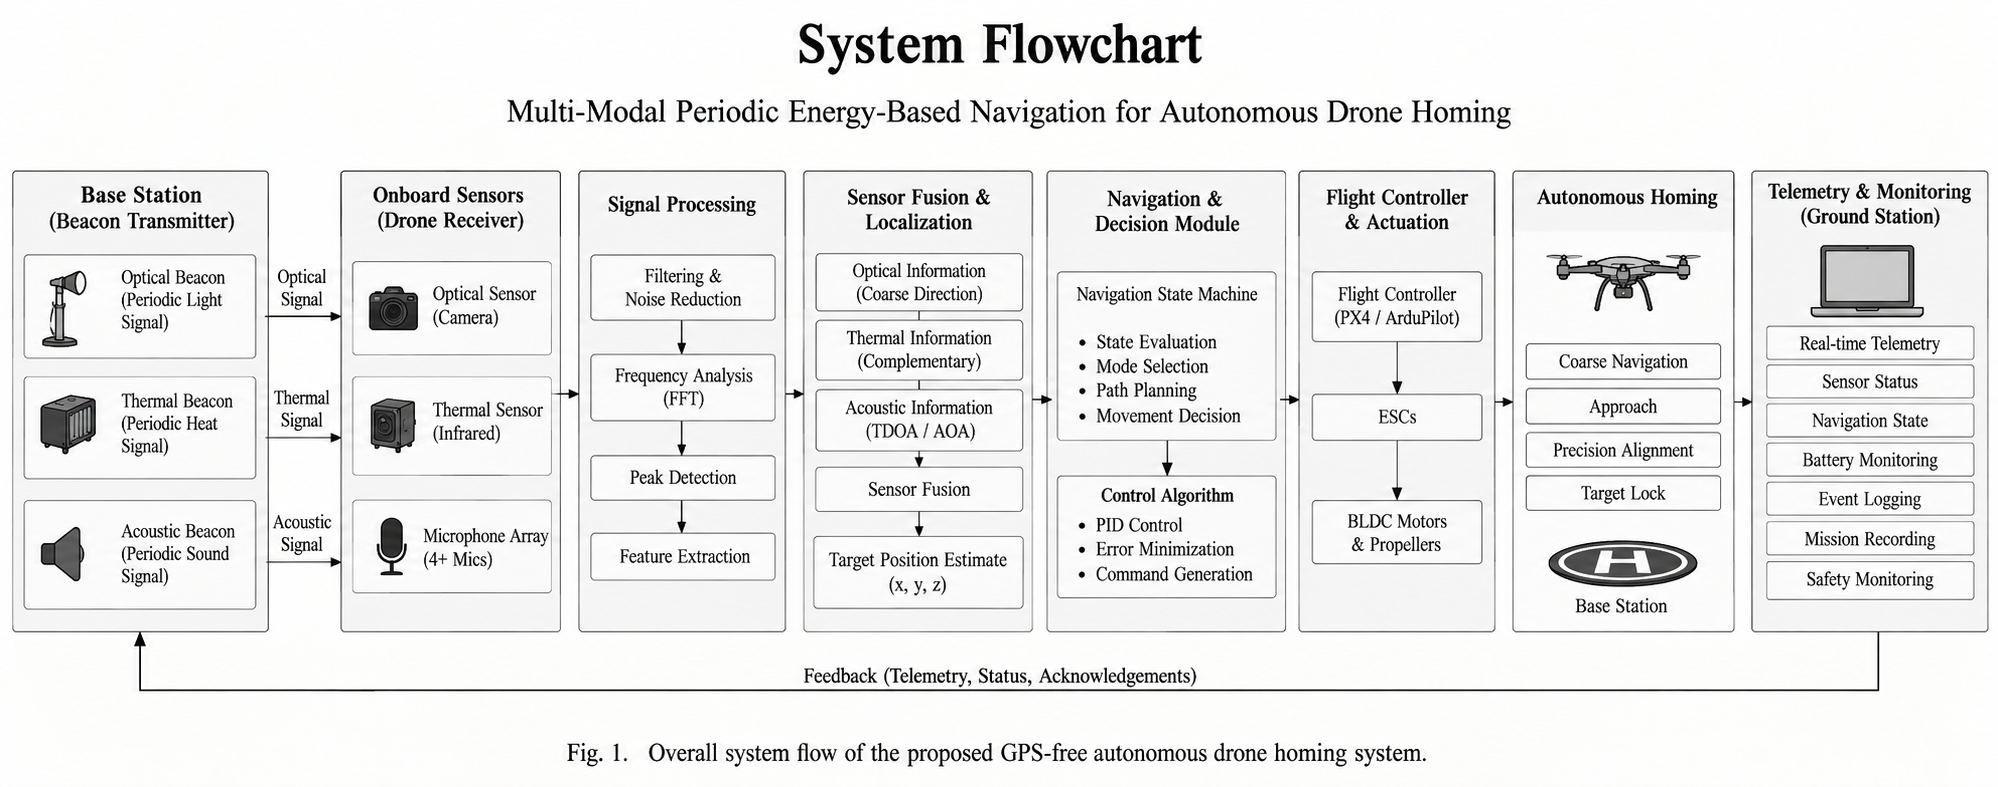
\includegraphics[width=0.9\textwidth]{system_flowchart.png}
\label{fig:system_flowchart}
\end{figure*}

% ---------------------------------------------------------
% BASE STATION
% ---------------------------------------------------------

\subsection{Base Station and Periodic Energy Beacon}

The base station acts as the explicit homing reference. It periodically emits
three identifiable signal classes: optical, thermal, and acoustic. The periodic
structure provides temporal information that helps distinguish the intended
beacon from unrelated environmental signals. Beacon parameters can include
carrier or modulation frequency, pulse period, intensity, duty cycle, and
transmission state.

Periodic beaconing is particularly useful in a reference-based architecture
because detection becomes a hypothesis-testing problem rather than an
open-ended search over the entire environment. The signal-processing layer can
correlate observations with expected temporal and spectral patterns before
passing them to the localization stage
\cite{oppenheim2010,haykin2014,knapp1976}.

% ---------------------------------------------------------
% SENSOR LAYER
% ---------------------------------------------------------

\subsection{Drone Sensor Layer}

The drone contains sensing elements matched to the three transmitted
modalities. The optical or infrared channel measures beacon intensity and
directional evidence. The thermal channel detects the thermal signature and
provides complementary information when visible-light conditions are
unfavorable. The acoustic channel uses a spatially separated microphone array
so that the same beacon event is observed at different sensor locations.

Microphone-array geometry is important because TDOA is converted into spatial
constraints through the known sensor separation and propagation velocity
\cite{brandstein2001,benesty2008,schmidt1986}. Sensor timestamps and sampling
rates must remain sufficiently synchronized for the expected localization
accuracy.

% ---------------------------------------------------------
% SIGNAL PROCESSING
% ---------------------------------------------------------

\subsection{Signal Processing and Feature Extraction}

Raw observations can contain environmental noise, multipath components,
reverberation, sensor noise, and irrelevant frequency content. The signal
processing stage therefore performs filtering, noise reduction, frequency
analysis, peak detection, and feature extraction.

For an acoustic signal $x(t)$, the continuous Fourier transform is

\begin{equation}
X(f)=\int_{-\infty}^{\infty}x(t)e^{-j2\pi ft}\,dt.
\end{equation}

The dominant frequency and spectral energy are compared with the expected
beacon signature. Classical digital signal-processing formulations provide the
frequency-domain and filtering foundations used in this stage
\cite{gonzalez2018,oppenheim1999,proakis2007,rabiner1975}.

A basic signal-to-noise ratio (SNR) measure is

\begin{equation}
SNR=10\log_{10}\left(\frac{P_s}{P_n}\right),
\end{equation}

where $P_s$ and $P_n$ are signal and noise power, respectively. For acoustic
localization, generalized cross-correlation and GCC-PHAT are appropriate tools
for estimating inter-channel delay under noise and reverberation
\cite{knapp1976,chen2006,do2010}.

% ---------------------------------------------------------
% LONG RANGE
% ---------------------------------------------------------

\subsection{Long-Range Optical and Thermal Homing}

During long-range navigation, optical and thermal observations provide coarse
direction toward the base station. The system does not require centimeter-level
accuracy at this stage; it requires a sufficiently reliable homing direction.
The navigation layer evaluates detection confidence, signal strength, and
consistency over successive observations.

The use of two complementary long-range modalities is intended to reduce the
probability that one environmental condition completely disables target
acquisition. Thermal sensing can provide useful information in low-light or
nighttime conditions, while optical sensing can provide stronger directional
cues when the beacon is visually distinct
\cite{jensen2007,thermal2026}.

% ---------------------------------------------------------
% NEAR FIELD
% ---------------------------------------------------------

\subsection{Near-Field Acoustic Localization}

When the estimated range reaches a predefined transition region, acoustic
localization is activated. For microphones $i$ and $j$, the TDOA is

\begin{equation}
\Delta t_{ij}=t_i-t_j.
\end{equation}

The corresponding path-length difference is

\begin{equation}
\Delta d_{ij}=c\Delta t_{ij},
\end{equation}

where $c$ is the speed of sound. Multiple microphone-pair measurements produce
multiple geometric constraints on the source direction. GCC-PHAT, SRP-PHAT,
AOA estimation, and hyperbolic localization can be used as progressively more
advanced implementations
\cite{knapp1976,brandstein2001,chen2006,do2010,srp2026,choi2020,liu2021,zhao2022}.

\begin{figure*}[!h]
\centering
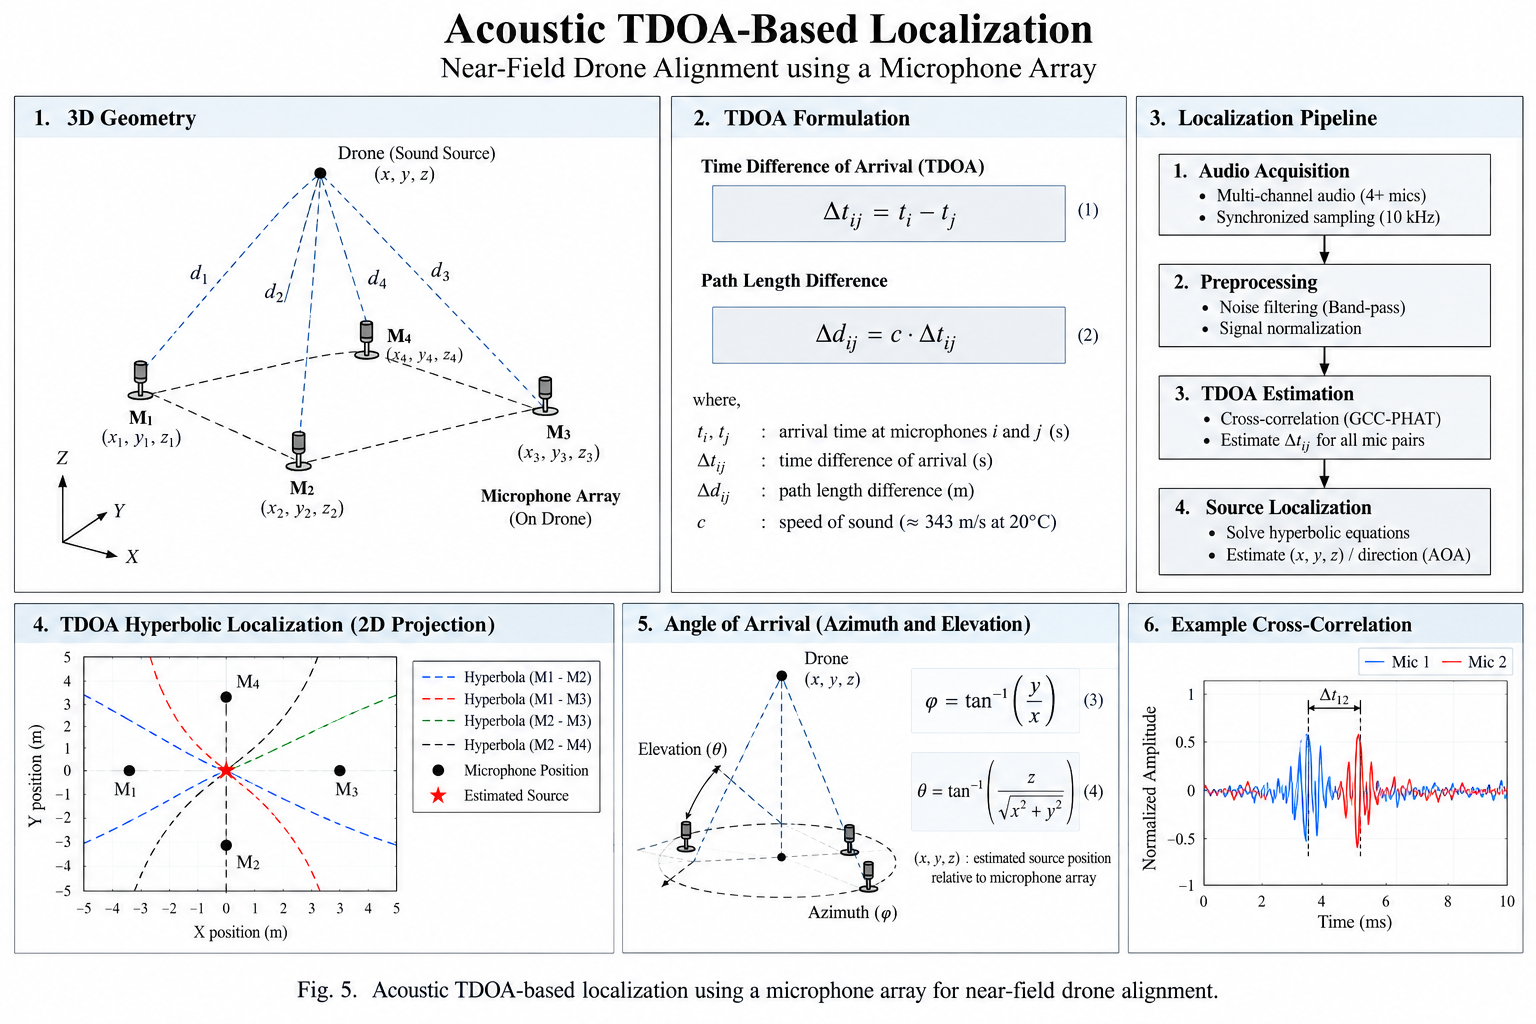
\includegraphics[width=0.9\textwidth]{tdoa_localization.png}
\label{fig:tdoa}
\end{figure*}

% ---------------------------------------------------------
% SENSOR FUSION
% ---------------------------------------------------------

\subsection{Sensor Fusion and Confidence Management}

The localization layer combines optical, thermal, and acoustic observations.
A generalized confidence-weighted estimate is expressed as

\begin{equation}
\hat{z}=w_o z_o+w_t z_t+w_a z_a,
\end{equation}

where $z_o$, $z_t$, and $z_a$ denote modality-specific measurements and the
weights satisfy an appropriate normalization. The weights are adjusted using
signal quality, noise level, detection confidence, and navigation mode.

For a practical implementation, the weights may be interpreted as normalized
inverse uncertainty or confidence scores. A Kalman or extended Kalman filter
can subsequently be introduced when a dynamic state model and covariance
estimates are available
\cite{kalman1960,welch1995,maybeck1979,barshalom2001,gustafsson2012,arun2020,barfoot2017,julier1997,dellaert2017,hall1997}.

% ---------------------------------------------------------
% MULTI MODAL METHODOLOGY
% ---------------------------------------------------------

\subsection{Multi-Modal Homing Methodology}

The complete homing procedure follows a staged strategy. Initially, the drone
searches for the periodic beacon and confirms the target using optical and
thermal observations. Once sufficient confidence is obtained, the system
enters coarse homing and progressively reduces the relative distance to the
base station. When the estimated range enters the predefined near-field
region, acoustic localization is activated. TDOA and AOA measurements then
provide additional directional information for final approach and alignment.
The process terminates when the target-lock condition satisfies the required
position and confidence thresholds.

\begin{figure*}[!h]
\centering
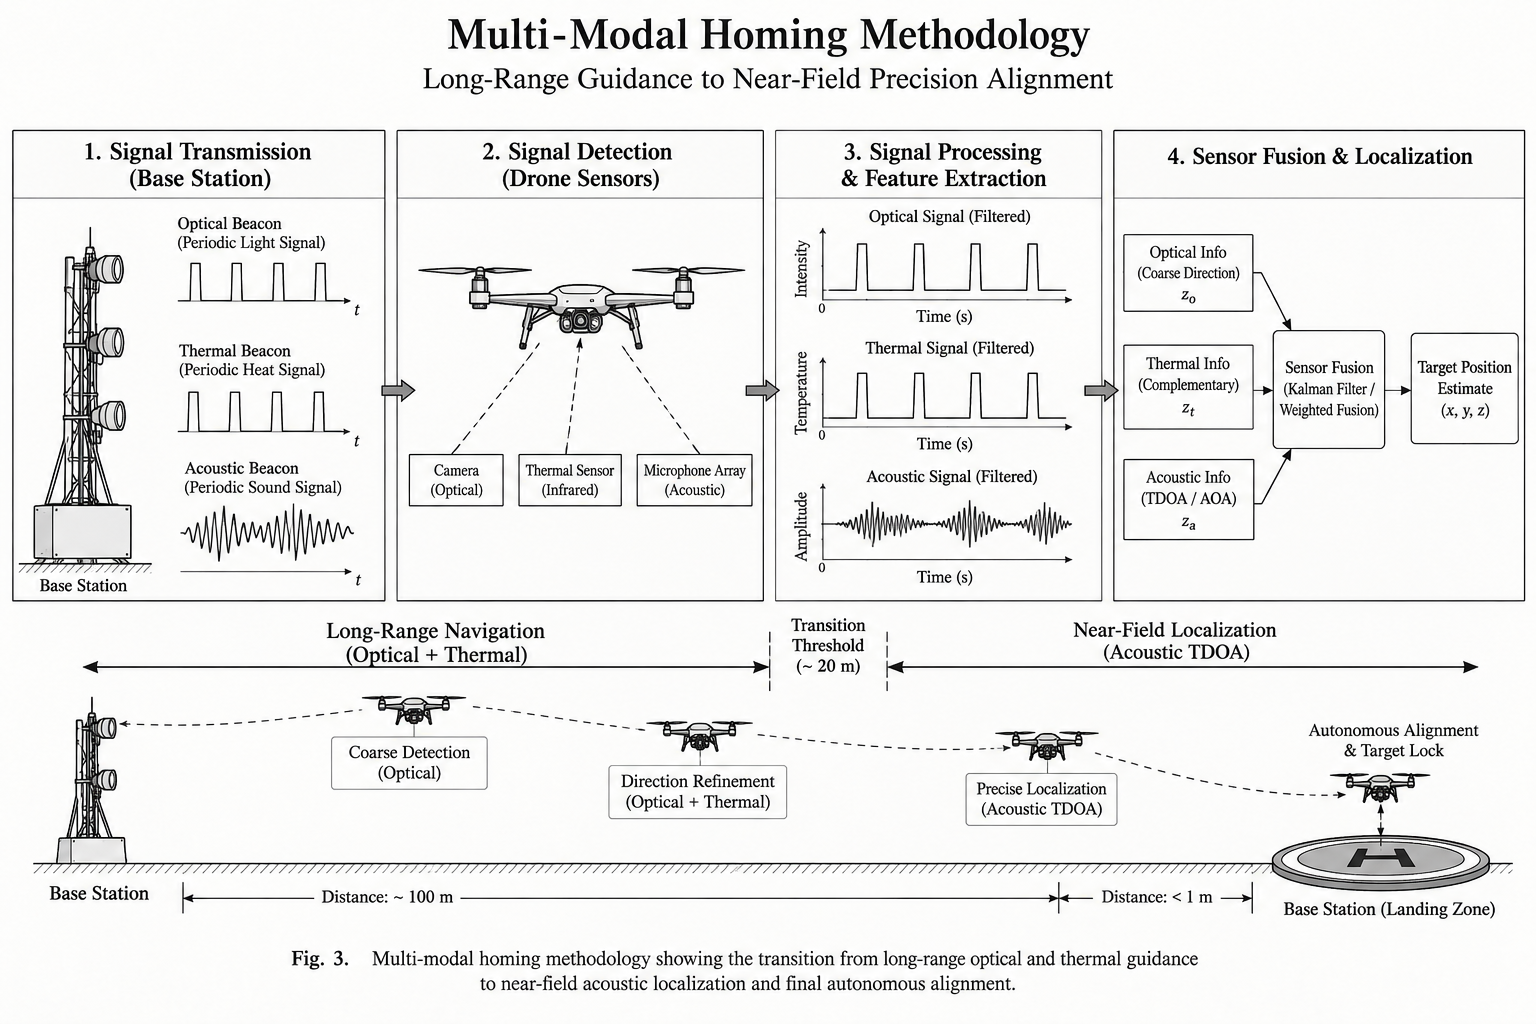
\includegraphics[width=0.9\textwidth]{homing_methodology.png}
\label{fig:homing_methodology}
\end{figure*}

% ---------------------------------------------------------
% NAVIGATION
% ---------------------------------------------------------

\subsection{Navigation State Machine and Control}

The navigation state machine contains system initialization, base-station
detection, optical acquisition, thermal confirmation, long-range localization,
coarse homing, near-field transition, acoustic localization, precision
alignment, target lock, and homing completion. Transitions depend on sensor
availability, signal quality, estimated distance, and localization confidence.

The controller generates desired heading, pitch, roll, and throttle corrections.
A PID controller is represented by

\begin{equation}
u(t)=K_pe(t)+K_i\int_0^t e(\tau)d\tau+
K_d\frac{de(t)}{dt},
\end{equation}

where $e(t)$ is the navigation error. PID and geometric control are established
approaches for multirotor stabilization and tracking
\cite{dorf2017,lee2010,mahony2012,bouabdallah2004,bouabdallah2007,hoffmann2007,lavretsky2013,slotine1991}.

\begin{figure*}[!h]
\centering
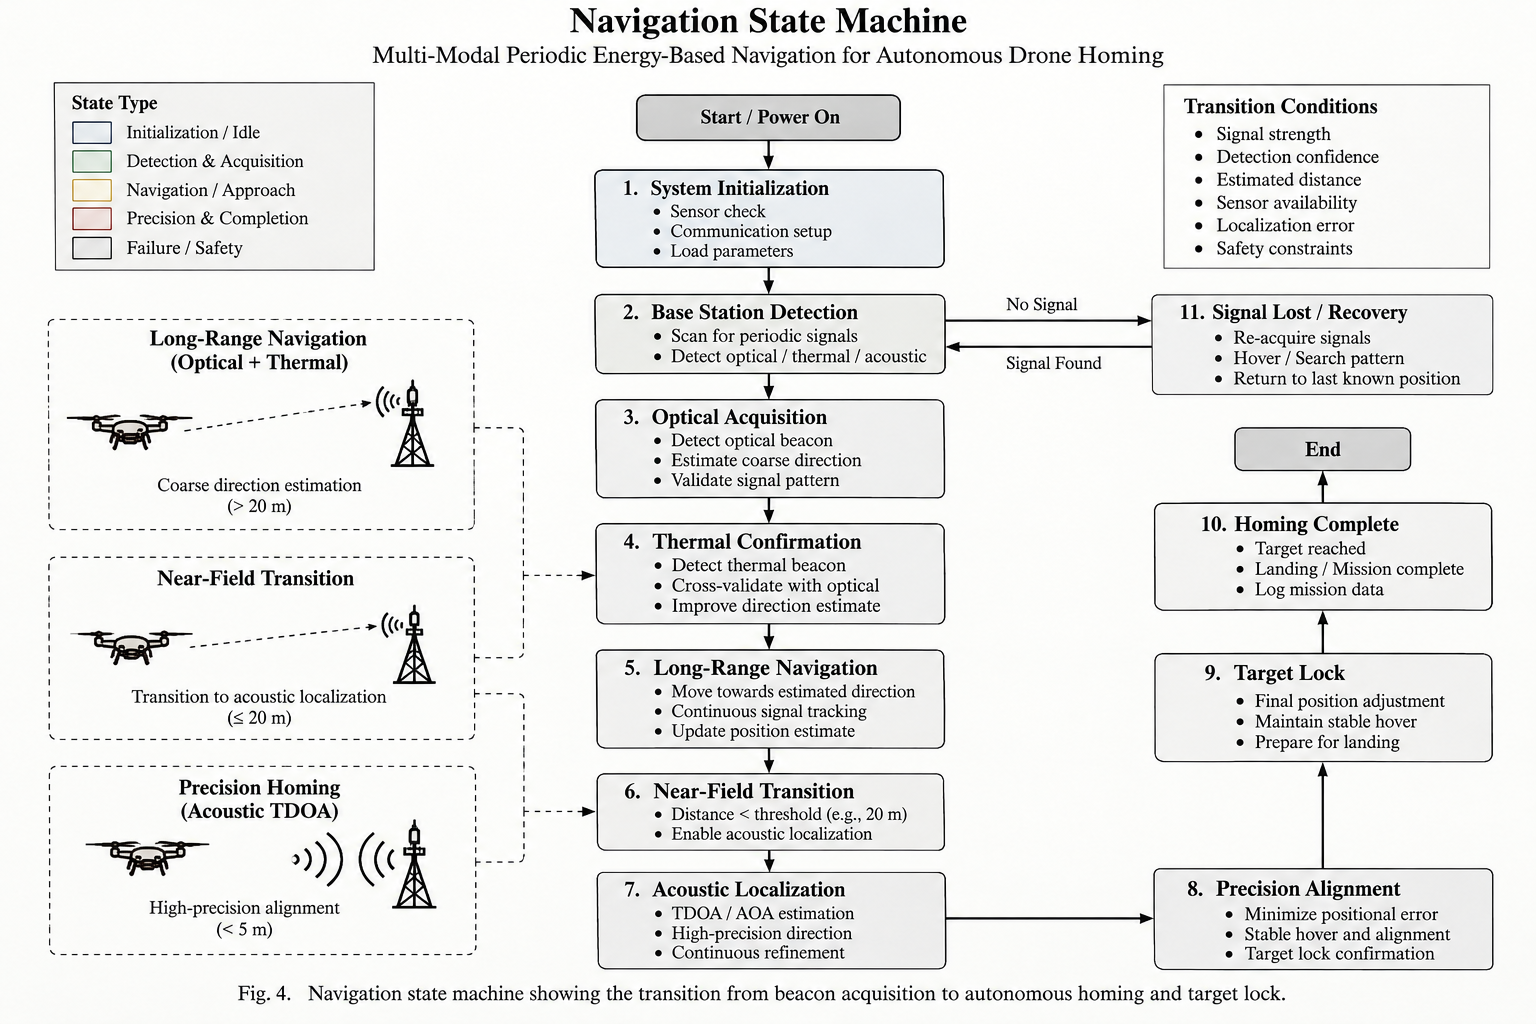
\includegraphics[width=0.9\textwidth]{navigation_state_machine.png}
\label{fig:navigation_state}
\end{figure*}

% ---------------------------------------------------------
% SYSTEM ARCHITECTURE DETAILS
% ---------------------------------------------------------

\subsection{System Architecture Details}

The major functional layers and their roles are summarized in
Table~\ref{tab:architecture}. The base-station layer generates the reference
signals, while the onboard sensing layer performs simultaneous acquisition of
the available physical modalities. The signal-processing layer converts raw
measurements into usable features and removes unwanted environmental
components. Localization and fusion then estimate the target state using
modality-specific measurements and confidence information.

The navigation layer determines the appropriate homing state and converts
the localization estimate into movement objectives. The flight-control layer
is responsible for stabilization and actuator timing, while the telemetry
layer provides mission observability. Finally, the safety layer monitors
critical system conditions and prevents the navigation loop from continuing
under unsafe or unreliable conditions.

The onboard processing platform may be an ESP32-class controller for lightweight
signal acquisition or a Raspberry Pi-class computer when greater processing
capacity is required. The flight controller remains responsible for low-level
stabilization and actuator timing.

\begin{table}[H]
\centering
\caption{Major System Components}
\label{tab:architecture}
\small
\begin{tabular}{p{2.25cm}p{5.0cm}}
\toprule
\textbf{Layer} & \textbf{Function} \\
\midrule
Base Station & Periodic optical, thermal, and acoustic beacon generation \\
Sensor Acquisition & Collection of optical, thermal, and acoustic measurements \\
Signal Processing & Filtering, FFT, noise reduction and feature extraction \\
Localization & AOA, TDOA and signal-strength based estimation \\
Sensor Fusion & Combination of multi-modal measurements \\
Navigation & Homing state selection and movement decision \\
Flight Control & PID/control commands for drone movement \\
Actuation & ESC, BLDC motor and propeller control \\
Telemetry & Monitoring of flight and sensor parameters \\
Safety & Detection of faults, signal loss and critical conditions \\
\bottomrule
\end{tabular}
\end{table}

\begin{figure*}[!h]
\centering
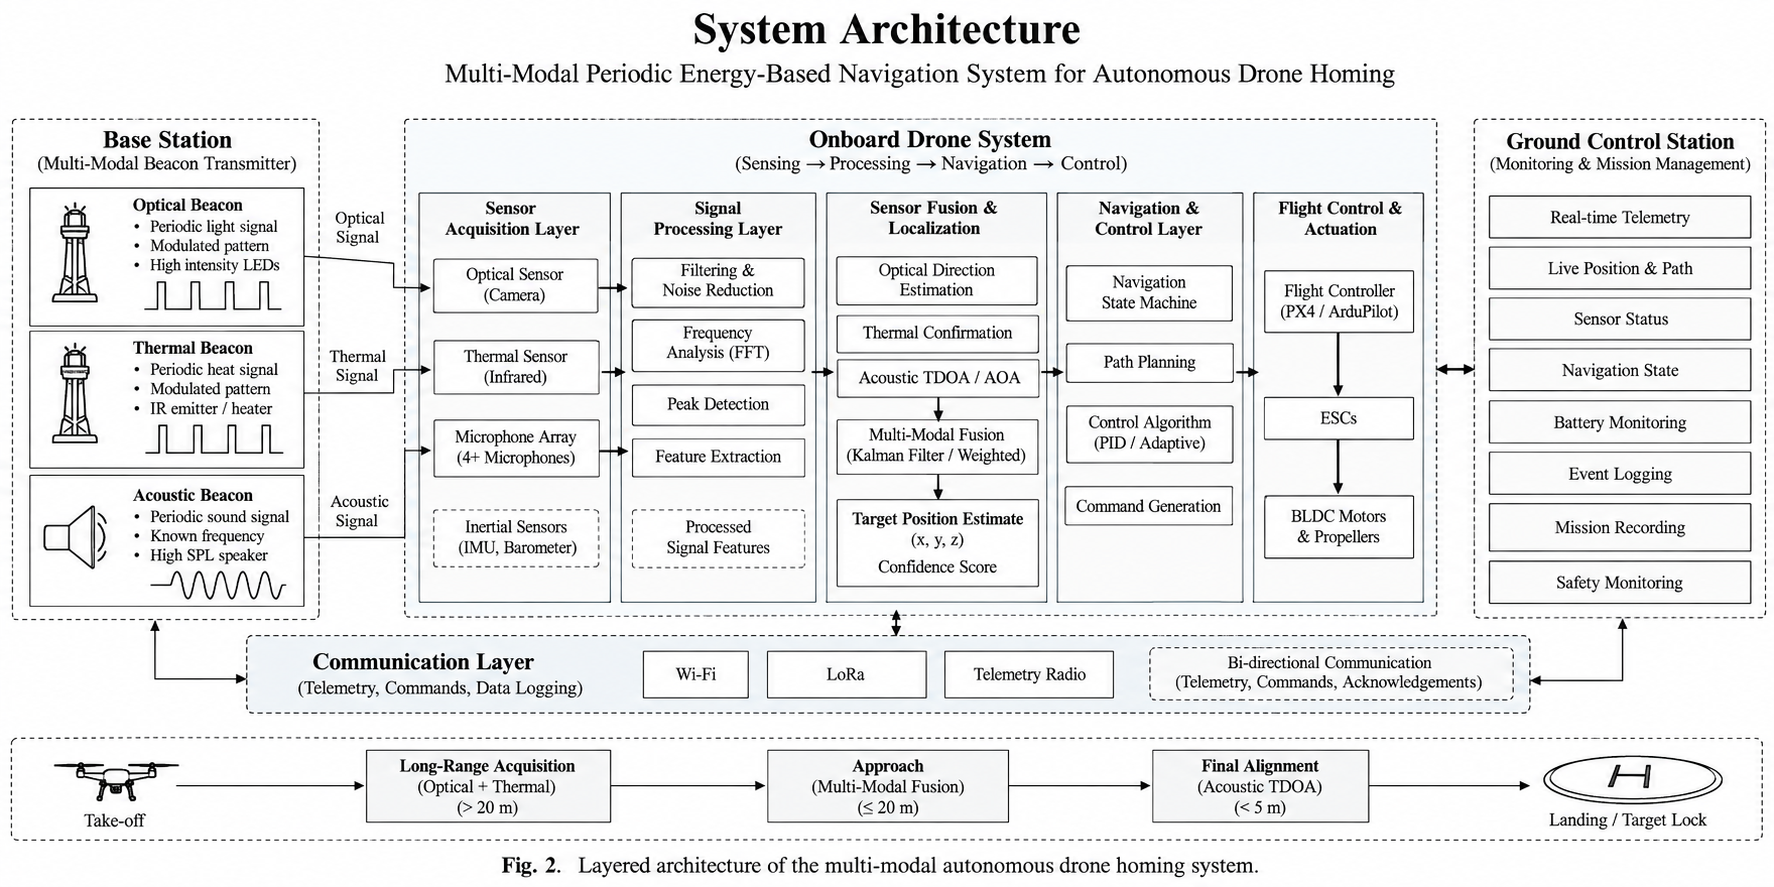
\includegraphics[width=0.9\textwidth]{system_architecture.png}
\label{fig:system_architecture}
\end{figure*}

% ---------------------------------------------------------
% GROUND CONTROL
% ---------------------------------------------------------

\subsection{Ground Control and Telemetry}

The ground-control station provides a unified monitoring layer for mission
state, sensor status, localization, flight telemetry, communication health,
battery state, and historical mission data. The displayed information includes
drone position and target direction, optical, thermal, and acoustic signal
strength, TDOA and AOA measurements, localization confidence, battery state,
flight attitude, motor telemetry, communication latency, packet loss,
navigation state, and fault logs.

A centralized telemetry provider allows the visualization layer to consume live
hardware data, replayed missions, or development streams without changing the
user interface. Mission history can contain identifiers, timestamps,
navigation states, localization measurements, signal information,
communication events, and system-health information. Telemetry replay is
useful for deterministic software validation before free-flight testing
\cite{mavlink2023,px4guide,ros2design}.

% ---------------------------------------------------------
% SECURITY
% ---------------------------------------------------------

\subsection{Security, Privacy and Safety}

The ground-control interface should implement authenticated access and
role-based authorization. Sensitive operations such as ARM, DISARM, START, and
ABORT should require appropriate authorization. Communications between the
drone, base station, and ground station should use authenticated and encrypted
channels where supported. Security controls should also protect telemetry and
mission history from unauthorized modification
\cite{nist80053,owasp2021}.

Safety monitoring continuously evaluates battery state, sensor availability,
communication quality, localization confidence, and critical faults. If
communication is lost or localization becomes unreliable, the system should
enter a predefined safe state rather than continuing uncontrolled navigation.
The distinction is important because standard autopilot return-to-home modes
may themselves require a valid global position estimate; therefore a GPS-free
homing architecture needs its own explicit fallback logic
\cite{px4return,px4failsafe}.

% =========================================================
% V. IMPLEMENTATION
% =========================================================

\section{Implementation and Technology Stack}

The prototype uses an embedded processing and flight-control stack together
with a web-oriented telemetry layer. The proposed technology stack is shown in
Table~\ref{tab:technology}.

\begin{table}[H]
\centering
\caption{Proposed Technology Stack}
\label{tab:technology}
\small
\begin{tabular}{p{2.3cm}p{4.9cm}}
\toprule
\textbf{Category} & \textbf{Technology} \\
\midrule
Embedded Processing & ESP32 / Raspberry Pi \\
Programming & C/C++, Python \\
Signal Processing & MATLAB, Python, FFT, digital filtering \\
Localization & AOA, TDOA, signal-strength analysis \\
Control & PID / adaptive control \\
Flight Hardware & Flight Controller, ESC, BLDC Motors \\
Sensors & Optical/IR, Thermal, Microphone Array \\
Communication & Wi-Fi / LoRa / Serial \\
Ground Station & React / Next.js, TypeScript \\
Visualization & Recharts / custom telemetry plots \\
Data & CSV, JSON, KML \\
Development & VS Code, Git, GitHub \\
Security Testing & Wireshark, OWASP ZAP, Postman \\
\bottomrule
\end{tabular}
\end{table}

\begin{figure*}[!h]
\centering
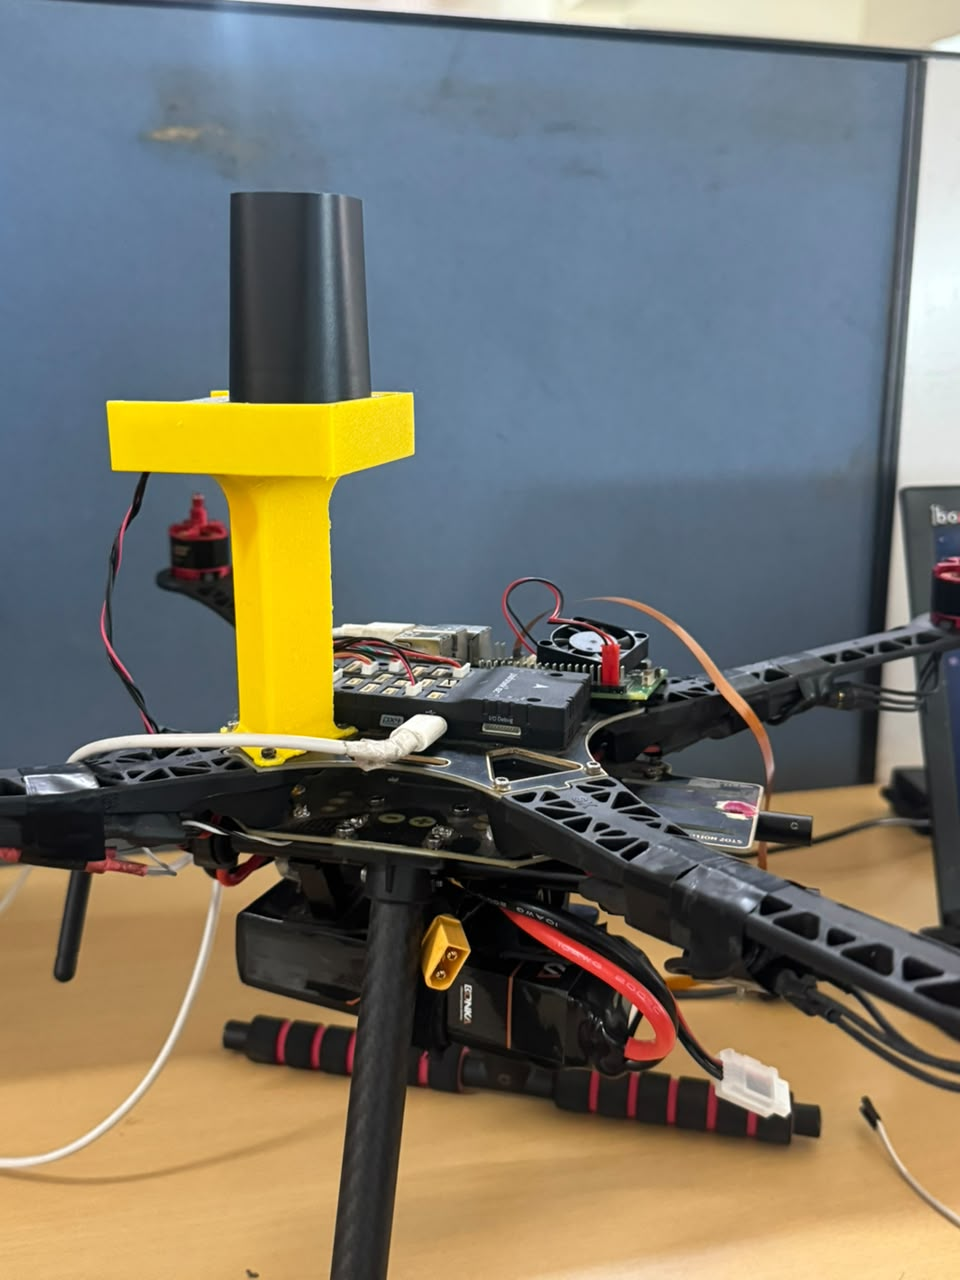
\includegraphics[width=0.6\textwidth]{implementation1.png}
\label{fig:implementation1}
\end{figure*}

\begin{figure*}[!h]
\centering
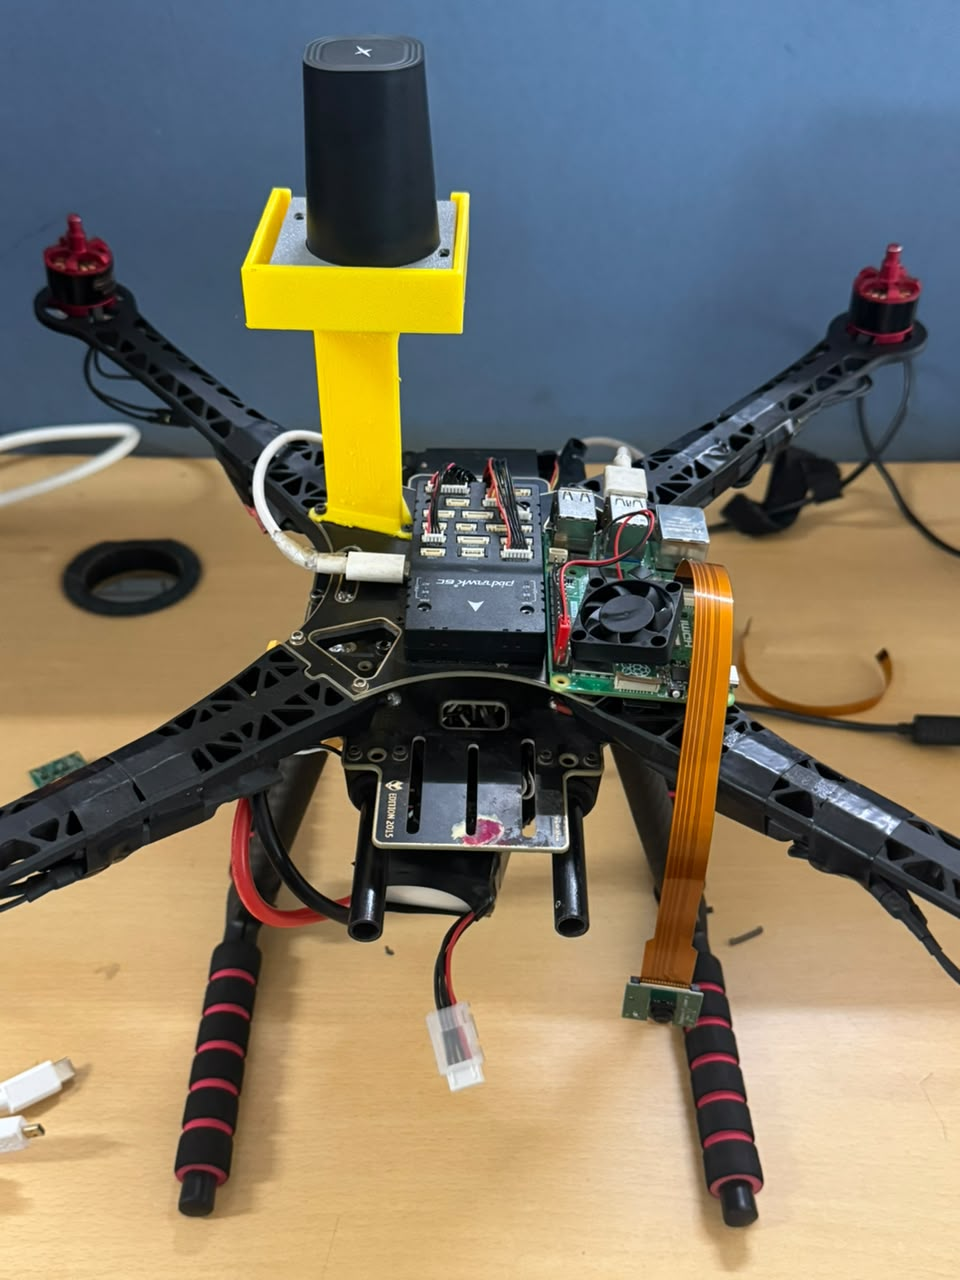
\includegraphics[width=0.42\textwidth]{implementation2.png}
\hfill
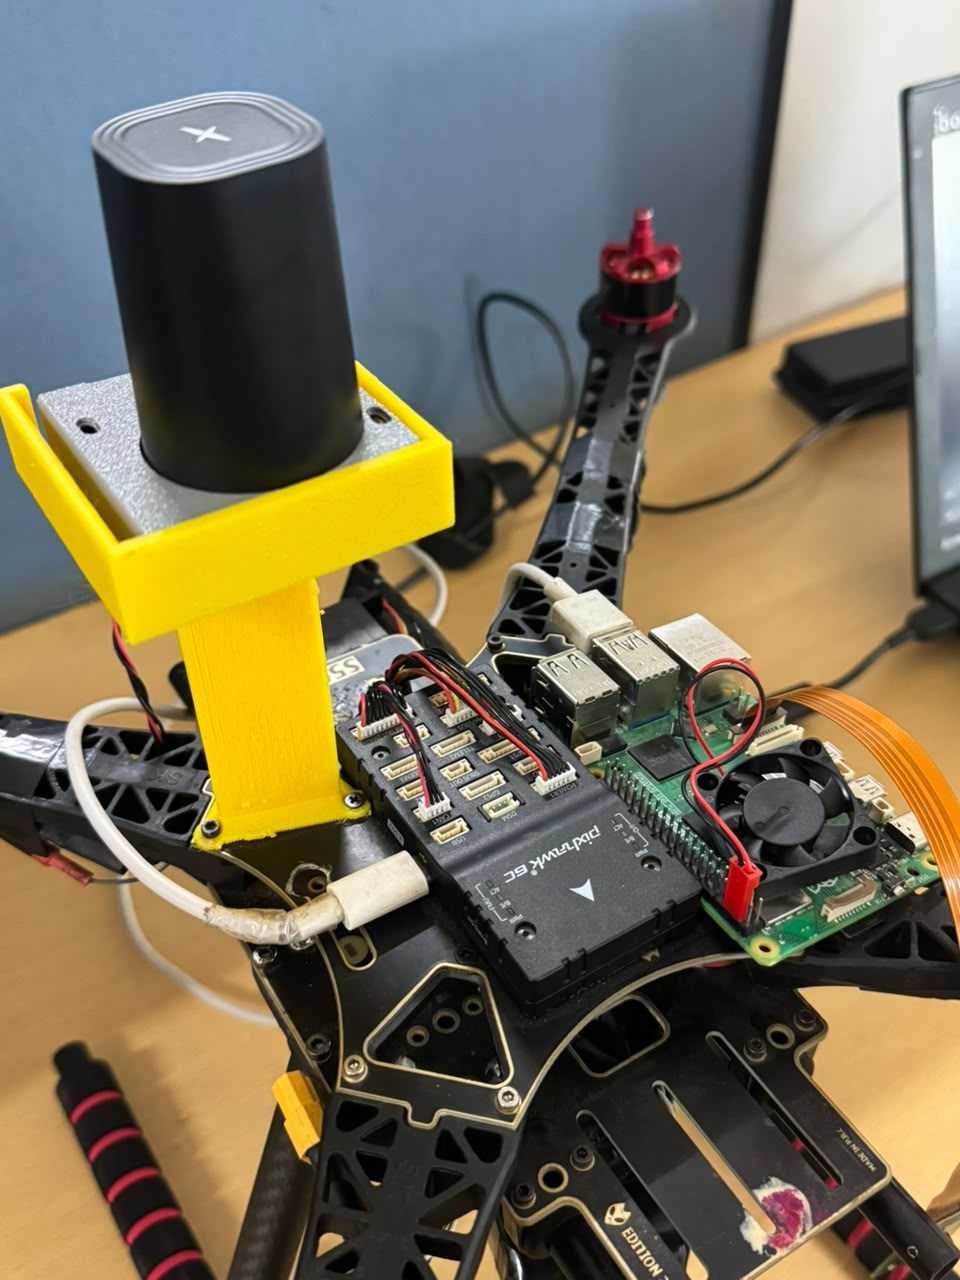
\includegraphics[width=0.42\textwidth]{implementation3.png}
\label{fig:implementation2}
\end{figure*}

The software architecture separates data acquisition from visualization. A
telemetry provider exposes a common interface for live hardware data, recorded
mission data, and development data, allowing the same ground-control interface
to be used throughout the development lifecycle.

% =========================================================
% VI. EXPERIMENTAL RESULTS AND ANALYSIS
% =========================================================

\section{Experimental Results and Analysis}

The evaluation is divided into signal-level, localization-level,
integration-level, telemetry-level, and homing-level observations. The current
paper reports development and replay observations from the implemented
software workflow and prototype integration. These values must not be
interpreted as statistically complete free-flight validation; controlled
flight experiments remain a required next step.

\subsection{Evaluation Metrics}

The principal evaluation metrics are localization error, signal-to-noise ratio,
detection confidence, fused confidence, homing success rate, navigation update
rate, telemetry rate, latency, and packet loss.

Localization error is defined as the Euclidean distance between the reference
and estimated target positions:

\begin{equation}
E=\sqrt{(x-\hat{x})^2+(y-\hat{y})^2+(z-\hat{z})^2}.
\end{equation}

SNR evaluates the ratio of detected beacon power to noise power. Detection
confidence represents the confidence assigned to the detected beacon after
modality-specific processing, while fused confidence represents the confidence
after combining the active modality estimates. Homing success rate represents
the percentage of replay scenarios reaching the defined target-alignment
condition. Navigation update rate measures the number of localization and
navigation decisions generated per second. Telemetry rate, latency, and packet
loss characterize communication and monitoring performance.

\subsection{Development and Replay Results}

Table~\ref{tab:results} retains the observations from the current development
stage. They are presented as engineering observations rather than claims of
final field performance.

\begin{table}[H]
\centering
\caption{Development and Replay Observations}
\label{tab:results}
\small
\begin{tabular}{p{3.6cm}c}
\toprule
\textbf{Parameter} & \textbf{Observation} \\
\midrule
Initial Homing Range & 100 m \\
Near-Field Transition & 20 m \\
Final Alignment & 0.8 m \\
Navigation Update Rate & 10 Hz \\
Fused Confidence & 92.4\% \\
Average Localization Error & 1.5 m \\
Homing Success in Replay Scenarios & $\approx$90\% \\
Telemetry Rate & 10--20 Hz \\
\bottomrule
\end{tabular}
\end{table}

The telemetry sequence demonstrates a staged reduction in relative distance.
During the initial phase, optical and thermal measurements support coarse
homing. As the estimated distance approaches the near-field threshold, the
acoustic stage is activated. The TDOA stage then contributes directional
information for final alignment. This behavior is consistent with the intended
architecture in which different modalities dominate at different navigation
stages.

\subsection{Signal and Localization Analysis}

Signal-processing performance is assessed using frequency detection, SNR,
peak detection, and filtering behavior. Known target positions can be used to
calculate AOA/TDOA localization error. Future controlled experiments should
evaluate the same metric over repeated trials under different noise, lighting,
temperature, distance, and reverberation conditions.

The current average localization error of 1.5 m is therefore a
development/replay observation, not a certified flight-test accuracy.
Likewise, the 92.4\% fused confidence represents the internal confidence
measure used by the current workflow and should not be equated directly with
probability of true position correctness.

\subsection{Integration and Telemetry Analysis}

The complete chain is evaluated as

{\small
\begin{center}
Sensor Data $\rightarrow$ Processing $\rightarrow$ Localization
$\rightarrow$ Navigation $\rightarrow$ Control.
\end{center}
}

Communication testing considers packet rate, latency, packet loss, and
reconnection behavior. The telemetry architecture also maintains temporal
consistency between distance, signal strength, localization confidence,
navigation state, and event history. This is important because independently
generated values can produce misleading demonstrations even when each value is
numerically plausible.

\subsection{Prototype Observation}

The implemented UAV prototype and sensor assembly shown in
Figs.~\ref{fig:implementation1} and~\ref{fig:implementation2} demonstrate the
physical integration direction of the project. The prototype should be treated
as a hardware-integration milestone rather than evidence that the full
multi-modal flight loop has already been validated under all environmental
conditions.

% =========================================================
% VII. COMPARATIVE ANALYSIS
% =========================================================

\section{Comparative Analysis}

To position the proposed system against representative GPS-denied or homing
approaches, Table~\ref{tab:comparison} provides a qualitative
architecture-level comparison. The comparison is intentionally based on design
characteristics reported in the literature rather than claiming identical
benchmark conditions.

\begin{table*}[t]
\centering
\caption{Qualitative Comparison of Representative UAV Navigation and Homing Approaches}
\label{tab:comparison}
\small
\begin{tabular}{p{2.8cm}p{3.3cm}p{3.3cm}p{3.3cm}p{3.5cm}}
\toprule
\textbf{Criterion} &
\textbf{GPS/GNSS-based RTH} &
\textbf{Vision/VIO/SLAM} &
\textbf{RF/UWB Localization} &
\textbf{Proposed Multi-Modal Homing} \\
\midrule
Primary Reference &
Satellite/global position &
Scene features and motion &
Anchors/beacons &
Dedicated periodic multi-modal beacon \\

GNSS Dependence &
High &
None during local operation &
None &
None \\

Infrastructure &
Satellite visibility &
Camera/environment &
Anchors/infrastructure generally required &
One designated base station \\

Long-Range Target Acquisition &
Strong when GNSS is valid &
Environment dependent &
Strong within radio coverage &
Optical + thermal coarse guidance \\

Near-Field Directional Refinement &
Limited by GNSS resolution/use case &
Strong if visual features remain trackable &
Strong with suitable geometry &
Acoustic TDOA/AOA refinement \\

Low-Light Robustness &
Independent of illumination &
Potentially reduced &
Independent of illumination &
Thermal channel provides complementary cue \\

RF Interference Sensitivity &
Vulnerable to GNSS interference/jamming &
Low &
Potentially significant &
Low for the core homing cues \\

Acoustic Noise Sensitivity &
Low &
Low &
Low &
Present in acoustic near-field stage \\

Drift Tendency &
Low when GNSS is healthy &
Can accumulate without global correction &
Low to moderate depending on estimator &
Bounded by external beacon observations \\

Main Limitation &
GNSS denial/obstruction &
Illumination, texture, compute &
Propagation, anchors, multipath &
Calibration, beacon dependency, environmental noise \\

System-Level Contribution &
Global navigation &
Local perception/localization &
Absolute/relative localization &
Staged sensing + fusion + homing + telemetry \\

\bottomrule
\end{tabular}
\end{table*}

GNSS return-to-home is mature and widely supported by autopilot stacks, but
standard return modes can require a valid global position estimate
\cite{px4guide,px4return}. Vision/VIO/SLAM avoids GNSS dependence and can provide
rich local geometry, but its robustness is linked to visual observability and
computational resources
\cite{leutenegger2015,forster2017,orbslam3}. UWB and related RF localization
can provide high-accuracy local positioning, but anchor configuration and
propagation conditions become important system constraints
\cite{zafari2019,wang2024}. The proposed architecture instead trades the
universality of map-based navigation for a deliberately installed homing
reference and complementary energy modalities.

The principal advantage of the proposed approach is therefore architectural:
it does not require every modality to solve the complete navigation problem.
Optical and thermal sensing handle target acquisition, while acoustic sensing
is reserved for a near-field precision role. This staged allocation can reduce
unnecessary computation and provides explicit failure points for monitoring.
The trade-off is the requirement for a designated beacon and careful sensor
calibration.

% =========================================================
% VIII. LIMITATIONS
% =========================================================

\section{Limitations}

The proposed system has several limitations. First, acoustic localization can
be affected by environmental noise, reflections, and reverberation
\cite{brandstein2001,chen2006}. Second, optical detection can be affected by
visibility and illumination, while thermal detection can be influenced by
ambient temperature, thermal clutter, and competing heat sources
\cite{jensen2007,thermal2026}.

The system currently depends on a designated beacon source. The base station
therefore has to be positioned and configured for the intended environment.
Unlike map-based VIO/SLAM approaches, the method does not attempt to infer a
complete global map, so it is not a universal replacement for general-purpose
navigation
\cite{orbslam3,thrun2005}.

Experimental calibration is also necessary. Sensor alignment, microphone-array
geometry, beacon characteristics, filtering parameters, confidence thresholds,
and controller gains can materially affect performance. Finally, the current
numerical results are development/replay observations. Physical validation is
required to determine actual range, accuracy, latency, energy consumption,
reliability, and robustness under wind, vibration, multipath, thermal clutter,
and obstruction.

% =========================================================
% IX. FUTURE SCOPE
% =========================================================

\section{Future Scope}

Future development will focus on physical integration and calibration of the
optical, thermal, and acoustic sensors with the flight controller, followed by
real-time embedded implementation of signal processing and TDOA/AOA
localization. Advanced state-estimation methods such as Kalman filtering,
extended Kalman filtering, and nonlinear estimation can be incorporated to
improve confidence-aware sensor fusion
\cite{welch1995,arun2020}. AI-based signal classification can also be explored
to distinguish beacon signals from environmental interference, while adaptive
transition thresholds can be introduced according to signal quality and
localization uncertainty.

Further work can improve beacon transmitter and receiver design to extend the
effective detection range and support multi-drone or multi-base-station
operation. Secure authenticated telemetry and command channels can be expanded
to strengthen operational safety. Hardware-in-the-loop testing should precede
controlled indoor and outdoor GPS-denied flight experiments so that timing,
calibration, estimator, and control failures can be identified before free
flight. Finally, onboard computation, payload, and power consumption can be
optimized to improve the practicality of the complete autonomous platform
\cite{faessler2018,px4guide,ros2design}.

% =========================================================
% X. CONCLUSION
% =========================================================

\section{Conclusion}

This paper presented a multi-modal periodic energy-based navigation system for
GPS-independent autonomous drone homing. The architecture combines optical,
thermal, and acoustic sensing so that each modality contributes at the stage
where it is most useful. Optical and thermal sensing support long-range target
acquisition, while microphone-array TDOA/AOA processing provides near-field
directional refinement. A confidence-aware fusion layer connects these
measurements to navigation states, closed-loop control, telemetry, and safety
monitoring.

The current development and replay observations show a structured workflow
with a 100 m initial homing range, a 20 m near-field transition, 0.8 m final
alignment, 10 Hz navigation updates, 92.4\% fused confidence, 1.5 m average
localization error, approximately 90\% replay homing success, and 10--20 Hz
telemetry. These figures are explicitly development-stage observations and
require physical flight validation before being treated as general performance
claims.

The principal contribution is therefore the system-level staged integration of
periodic optical, thermal, and acoustic homing cues into a complete navigation
architecture. The next phase is controlled hardware-in-the-loop and flight
experimentation under realistic noise, obstruction, lighting, thermal, and
communication conditions.

% =========================================================
% REFERENCES
% =========================================================

\bibliographystyle{IEEEtran}
\bibliography{ref}

\balance

\end{document}